%%%% Document setup
\documentclass[a4paper,landscape,title page]{article}
\setlength{\oddsidemargin}{-0.65in}	% default=0in
\setlength{\textwidth}{11in}		% default=9in
\setlength{\textheight}{6.85in}		% default=5.15in
\setlength{\topmargin}{-1.0in}		% default=0.20in
\setlength{\headsep}{0.35in}		% default=0.35in
\setlength{\parskip}{1.2ex}
\setlength{\parindent}{0mm}

%%%% Use packages
\usepackage{times}
\usepackage{tikz,pgf}
\usetikzlibrary{arrows,automata,trees,plotmarks,calc}


%%%%
\title{Goal-Plan hierarchy for test \textit{Hanoi Towers}}
\author{
Dhirendra Singh\\
dhirendra.singh@rmit.edu.au}
\begin{document}
%\maketitle

\begin{figure*}[t]
\begin{center}

\begin{tikzpicture}[scale=1.0,level distance=1.5cm]
\tikzstyle{txt}=[scale=1.0]
\tikzstyle{planbox}=[scale=1.0,draw,minimum height=0.9cm,minimum width=1.0cm]
\tikzstyle{goalbox}=[scale=1.0,draw,rounded corners,minimum height=0.9cm,minimum width=1.0cm]
\tikzstyle{level 1}=[sibling distance=6.0cm] 
\tikzstyle{level 2}=[sibling distance=5.0cm] 
\tikzstyle{level 3}=[sibling distance=3.0cm]
\tikzstyle{level 4}=[sibling distance=3.0cm]
\tikzstyle{level 5}=[sibling distance=1.5cm]
\tikzstyle{level 6}=[sibling distance=1.3cm]

\node[goalbox,yshift=1cm,solid] (T) {$G[1]$}
	child {node[planbox] {$P_3$}
		child {node[goalbox] {$G[2]$}
			child {node[planbox] {$P_3$}
				child {node[goalbox] {$G[4]$}
					child {node[planbox] {$P_3$}
						child[dashed] {node[goalbox] {$G[8]$}}
						child[dashed] {node[goalbox] {$G[4]$}}
					}
					child {node[planbox] {$P_{1/2}$}}
					child {node[planbox] {$P_4$}
						child[dashed] {node[goalbox] {$G[9]$}}
						child[dashed] {node[goalbox] {$G[4]$}}
					}
				}
				child[dashed] {node[goalbox] {$G[2]$}}
			}
			child {node[planbox] {$P_{1/2}$}}
			child {node[planbox] {$P_4$}
				child {node[goalbox] {$G[5]$}
					child {node[planbox] {$P_3$}
						child[dashed] {node[goalbox] {$G[10]$}}
						child[dashed] {node[goalbox] {$G[5]$}}
					}
					child {node[planbox] {$P_{1/2}$}}
					child {node[planbox] {$P_4$}
						child[dashed] {node[goalbox] {$G[11]$}}
						child[dashed] {node[goalbox] {$G[5]$}}
					}
				}
				child[dashed] {node[goalbox] {$G[2]$}}
			}
		}
		child[dashed] {node[goalbox] {$G[1]$}}
	}
	child {node[planbox] {$P_{1/2}$}}
	child {node[planbox] {$P_4$}
		child {node[goalbox] {$G[3]$}
			child {node[planbox] {$P_3$}
				child {node[goalbox] {$G[6]$}
					child {node[planbox] {$P_3$}
						child[dashed] {node[goalbox] {$G[12]$}}
						child[dashed] {node[goalbox] {$G[6]$}}
					}
					child {node[planbox] {$P_{1/2}$}}
					child {node[planbox] {$P_4$}
						child[dashed] {node[goalbox] {$G[13]$}}
						child[dashed] {node[goalbox] {$G[6]$}}
					}
				}
				child[dashed] {node[goalbox] {$G[3]$}}
			}
			child {node[planbox] {$P_{1/2}$}}
			child {node[planbox] {$P_4$}
				child {node[goalbox] {$G[7]$}
					child {node[planbox] {$P_3$}
						child[dashed] {node[goalbox] {$G[14]$}}
						child[dashed] {node[goalbox] {$G[7]$}}
					}
					child {node[planbox] {$P_{1/2}$}}
					child {node[planbox] {$P_4$}
						child[dashed] {node[goalbox] {$G[15]$}}
						child[dashed] {node[goalbox] {$G[7]$}}
					}
				}
				child[dashed] {node[goalbox] {$G[3]$}}
			}
		}
		child[dashed] {node[goalbox] {$G[1]$}}
	}
;

\end{tikzpicture}

\vskip 1.5cm
\caption{Goal-Plan hierarchy for \textit{Hanoi Towers} showing plan unfolding using bounded recursion with depth $d$. The top level goal ($G[1]$) is at $d=0$. Shown here is unolding upto $d=3$. All goals belongs to class $G$ with type $T$ represeted as $G[T]$. The total number of plans in the hierarchy is always $4$ --- the repetition at each level is purely to allow visualisation of the unfolding. Plans $P_1$ and $P_2$ are leaf plans and are shown as $P_{1/2}$ for brevity. For a puzzle with $9$ discs, $d=8$ will ensure sufficient recursion to ensure a solution is always found. Consequently, if a solution is not found in $d$ unfolds then we have made a bad move along the way and should be considered a failure. Note that in this domain a plan never fails per se, since a legal move can be made in every possible state.}
\end{center}
\end{figure*}

\end{document}
%%%%